%   Filename    : chapter_4.tex 
\chapter{Research Methodology}
This chapter presents the tools, techniques, and methodologies that was used for the development of TUKIB. This chapter also specifies the software and hardware requirements, as well as, the comprehensive processes included in creating the system.

\section{Research Activities}

\subsection{Development Framework}

\textbf{Agile Methodology}

The software development approach that the developers followed in developing TUKIB is the agile methodology. Agile methodology, or simply agile, is a framework that emphasizes iterative development and features communication and collaboration, adaptive planning, and continuous development (Agile Framework, 2022). The developers chose this framework because of its flexibility and adaptability to change, which is beneficial, especially with evolving user requirements. 

As seen from \figref{fig:agile}, agile involves continuously cycling through phases of development, testing, and review or feedback before finally launching the system. This enables developers to make adjustments and improvements based on user input. 

\begin{figure}[h]
	\centering 
	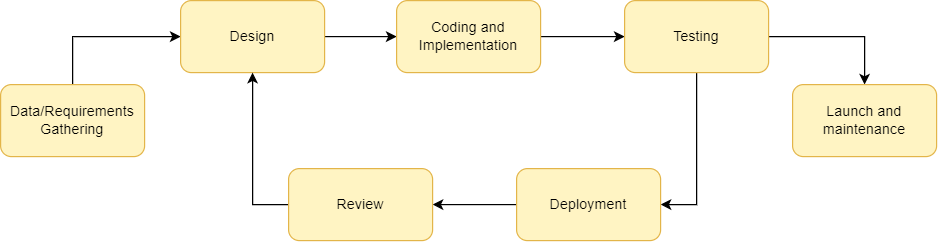
\includegraphics[width=1\textwidth]{agile methodology.png}
	\caption{Agile Methodology}
	\label{fig:agile}
\end{figure}

However, while Agile offers numerous benefits, it also has its caveats. One of the main challenges is that its iterative nature may lead to a lack of clear, long-term project goals, which can sometimes result in scope creep or unclear project direction. Agile can also require significant time and resources to maintain regular communication and collaboration, which may not always be feasible for teams with limited availability or tight schedules. Additionally, because Agile thrives on flexibility, it may be difficult to estimate and manage project timelines accurately. Finally, for larger teams or projects, scaling Agile to ensure coordination across different teams can be complex, and there may be difficulties in integrating Agile with other traditional project management frameworks. \newline

\textbf{Data Gathering and Documentation}

The developers began the project by visiting the UPV RRC, where they conducted interviews with stakeholders. This phase was essential for gaining a comprehensive understanding of the institution's specific needs and for planning the system features accordingly. The data gathered during these interviews guided the subsequent phases of the project, ensuring that the system is tailored to meet the requirements and expectations of its users. 

This phase includes the following activities:

\begin{itemize}
	\item \textbf{Defining Objectives.} Establishing the primary goals of TUKIB based on preliminary research and stakeholder input, ensuring that the project aligns with user needs.
	\item \textbf{Stakeholder Identification.} Identifying key stakeholders, including RRC personnel and potential users, to ensure that a diverse range of needs is considered and addressed throughout the development process.
	\item \textbf{Defining User Requirements.} Collecting and analyzing user requirements through interviews and interactions with stakeholders. This will involve creating user stories to capture the specific needs and expectations of different user groups, ensuring that the system design is informed based on real-world usage scenarios.
\end{itemize}

\textbf{System Design}

After data gathering, the system's architectural design was developed. This process involved creating a context model to outline the system's interactions with external entities. A process flow diagram was also constructed to detail the specific processes and workflows, while database models will be designed to ensure efficient data storage and retrieval. 

The researchers also focused on effective user interfaces (UI) for service request handling and management, investigating best practices and design principles that enhance user experience based on feedback from users of existing similar software or systems. Once all necessary information is gathered, a mock-up design of TUKIB was created, serving as the basis for the system's prototype. Together, these diagrams and designs provided a comprehensive framework that will guide the development and implementation of the system effectively.\newline

\textbf{Implementation}

From the design phase, the development of the system started. The frontend was built with the intention to ensure a user-friendly interface while the backend supports functionality through efficient data processing and secure user authentication. A chatbot was also integrated to facilitate real-time client support and interaction with the system.

Since the developers followed the Agile methodology, the implementation phase occured alongside testing. This iterative process involved cycles of development and testing during each sprint, with each sprint lasting two weeks. This approach allowed for continuous feedback and improvements, ensuring further that the system meets user needs effectively.\newline

\textbf{Testing}

The testing of the system consisted of 2 main components to ensure its reliability, usability, and overall performance.

\begin{itemize}
	\item \textbf{Alpha Testing.} During and after the development of each feature, extensive user testing was conducted to ensure that each feature works as intended. Any bugs or problems was immediately fixed. For features dependent on other features (i.e. user account creation must function correctly before user can log in), thorough testing ensured and verified that the integration between these features operates smoothly.
	
	\item \textbf{Beta Testing.}  Beta testing was be done with a limited group of users composed of available RRC staff and selected potential customers of RRC (e.g. students and faculty). This phase allowed real-world usage feedback and helped in identifying any remaining bugs and usability issues. Users tested the system in various environments and encouraged to provide insights on functionality, performance, and overall experience.\newline
\end{itemize}

\textbf{Deployment and Maintenance}

The final product of the study, TUKIB, will be made available to the intended users. In this phase, ongoing maintenance and regular performance monitoring, especially of the backend, are essential to ensure stability and reliability. Feedback forms will be issued to the users to gather their thoughts and insights about the system or to report any encountered bugs. Constant feedback from users during this phase will guide further improvements and updates.

While these activities are expected to occur during the deployment and maintenance phase, it is important to note that this phase is beyond the scope of the current study.

\section{Data Gathering}
The data gathering for the system requirements of TUKIB started with a comprehensive visit to the UPV RRC during the researchers' internship. This phase involved engaging with key personnel and understanding the intricacies of the center's operations. The following subsections detail the key activities and information gathered during this visit.

\subsection{Facility Tour}
During the visit, the researchers met with the center's director, administrative staff, and laboratory heads. This introduction provided valuable insights into the roles and responsibilities of various individuals and departments within the UPV RRC. Understanding these dynamics was crucial for tailoring the system to fit the institution's workflows.

The researchers were also given a guided tour, which provided an overview of various laboratories and services offered. These services include:

\begin{itemize}
	\item \textbf{Sample Processing.}The RRC provides sample processing services, essential for research and analysis.
	\item \textbf{Laboratory Equipment Rental} Various pieces of laboratory equipment are available for rent, which supports a wide range of scientific projects.
	\item \textbf{Training and Workshops.} The RRC offers training sessions on laboratory equipment, promoting user proficiency.
	\item \textbf{Facility Rental.} Spaces in the RRC like the Audio-Visual Room (AVR) and conference rooms, ideal for presentations, meetings, and events, are also available for rentals.
\end{itemize}

Each laboratory was introduced in detail, with specific equipment and services discussed in terms of their functionalities and purpose. The UPV RRC houses five (5) laboratories, namely: Biology, Microbiology, Nanotechnology, Applied Chemistry Laboratory, and Food, Feeds, and Functional Nutrition Laboratory.

\subsection{Stakeholder Identification and Engagement}
The success of workflow automation hinges on understanding the needs and expectations of its key stakeholders. These stakeholders include the RRC laboratory and administrative staff, the clients (university and student researchers and external users of the RRC facilities), the developers, and the member/s of the Computer Science Faculty guiding the project.

The researchers' interaction with the stakeholders allowed the gathering of valuable information on the existing system and the challenges that the institution faces. This feedback played a crucial role in shaping the direction of this study's system design, as it highlighted the need for automation, service tracking, and streamlined communication between stakeholders. Additionally, stakeholders were interviewed on their specific needs and pain points. These discussions led to the creation of user stories, which helped to contextualize the requirements from various perspectives. 

This in-depth exposure to the center’s operations was essential for the initial design and development phase of TUKIB, providing a strong foundation for creating a system tailored to the specific needs of the RRC.

\subsection{Scope and Limitations of UPV RRC Services}
Through discussions with the RRC staff, the researchers obtained a clear picture of the scope of services provided by the institution, as well as, the limitations is faces. Some of these limitations include:

\begin{itemize}
	\item The UPV RRC has no website available to the public which presents its mission, vision, services offered, as well as, steps or guide on how to request a service, and other relevant information. This limits clients from acquiring necessary information about the center and its services. The only platform that they utilize for disseminating news, activities, and information about their services is through a Facebook page which lacks structure and organization.
	\item The staff also has difficulty in managing and tracking equipment and facility availability in real-time, as it is essential to ensure seamless delivery of the institution's services.
	\item Manual service request and data management are also a problem as the RRC’s current system relies mainly on Google Forms and Sheets, which poses challenges in efficiency.
\end{itemize}

\section{System Requirements}

Based on the gathered data with stakeholders and observations during the facility tour, several key user requirements were identified for the development of TUKIB. 

\begin{itemize}
	\item \textbf{Service Information Accessibility}
	
	A website that allows clients or researchers to gain information about the UPV RRC and the services it provides, along with the steps on how to avail those services. 
	
	\item \textbf{Automated Service Requests}
	
	A system that automates the end-to-end flow of service request process, from submission of request to giving of feedback, in order to reduce the workload on staff and provide ease for clients.
	
	\item \textbf{Equipment and Facility Availability Tracking}
	
	A system that automates the tracking of the availability of equipment and facilities. This includes a calendar that tracks the facility availability schedule and an equipment inventory management system. 
	
	\item \textbf{Data Management and Reporting}
	
	A system for managing data related to client transactions, service requests, equipment use, and facility bookings. This system should support generating detailed reports for monitoring and decision-making.
	
	\item \textbf{User Account Management}
	
	A system to monitor client profiles and their transaction history with the UPV RRC, including payments, requests, and feedbacks.
	
	\item \textbf{Feedback Mechanism}
	A feedback mechanism that allows clients to complete a service feedback survey and automatically generate feedback statistics for easier feedback analysis.
	
\end{itemize}

With the data gathered, a checklist for all the features to be implemented was made. The purpose of this was to track and verify each feature during development and testing. Table~\ref{tab:requirements} lists down all the requirements and whether these requirements have been developed and achieved.

\newpage

\begin{table}[ht]
	\centering
	\begin{tabular}{|p{10cm}|c|}
		\hline
		\textbf{Requirements/Modules} & \textbf{Accomplished (Y/N)} \\
		\hline
		\multicolumn{2}{|l|}{\textbf{Backend Requirements}} \\
		\hline
		Local Database & \\
		Automatic archiving & \\
		RESTful API & \\
		Role-based access control & \\
		Error handling, validation, \& logging & \\
		\hline
		\multicolumn{2}{|l|}{\textbf{Privacy Requirements}} \\
		\hline
		User password encryption & \\
		Session or token authentication & \\
		Restriction of unauthorized access & \\
		Log in attempts limit/Brute-force protection & \\
		\hline
		\multicolumn{2}{|l|}{\textbf{User Interface Requirements}} \\
		\hline
		Client interface & \\
		Admin Staff interface & \\
		University Researcher interface & \\
		TECD Staff interface & \\
		Director interface & \\
		\hline
		\multicolumn{2}{|l|}{\textbf{Functional Requirements}} \\
		\hline
		User registration and authentication & \\
		Request tracking and management & \\
		Feedback mechanism & \\
		Notification system & \\
		Calendar system & \\
		Chatbot for FAQs and initial consultation & \\
		End-to-end flow of service request process & \\
		\hline
		\multicolumn{2}{|l|}{\textbf{UI/UX Design Requirements}} \\
		\hline
		Responsive design & \\
		User-friendly navigation & \\
		Feedback/confirmation messages & \\
		\hline
	\end{tabular}
	\caption{System Requirements Checklist}
	\label{tab:requirements}
\end{table}

\section{System Design}

\subsection{Process Flow Diagram}

\figref{fig:process_flow} illustrates the complete service delivery process of the UPV RRC through TUKIB. The process begins with an initial consultation with the RRC. Once the consultation is approved, users can create an account and submit a service request. The workflow then proceeds through several stages, including review and approval, execution of the service, and concludes with collecting feedback from the client—providing opportunities for continuous improvement.

\begin{figure}[h]
	\centering 
	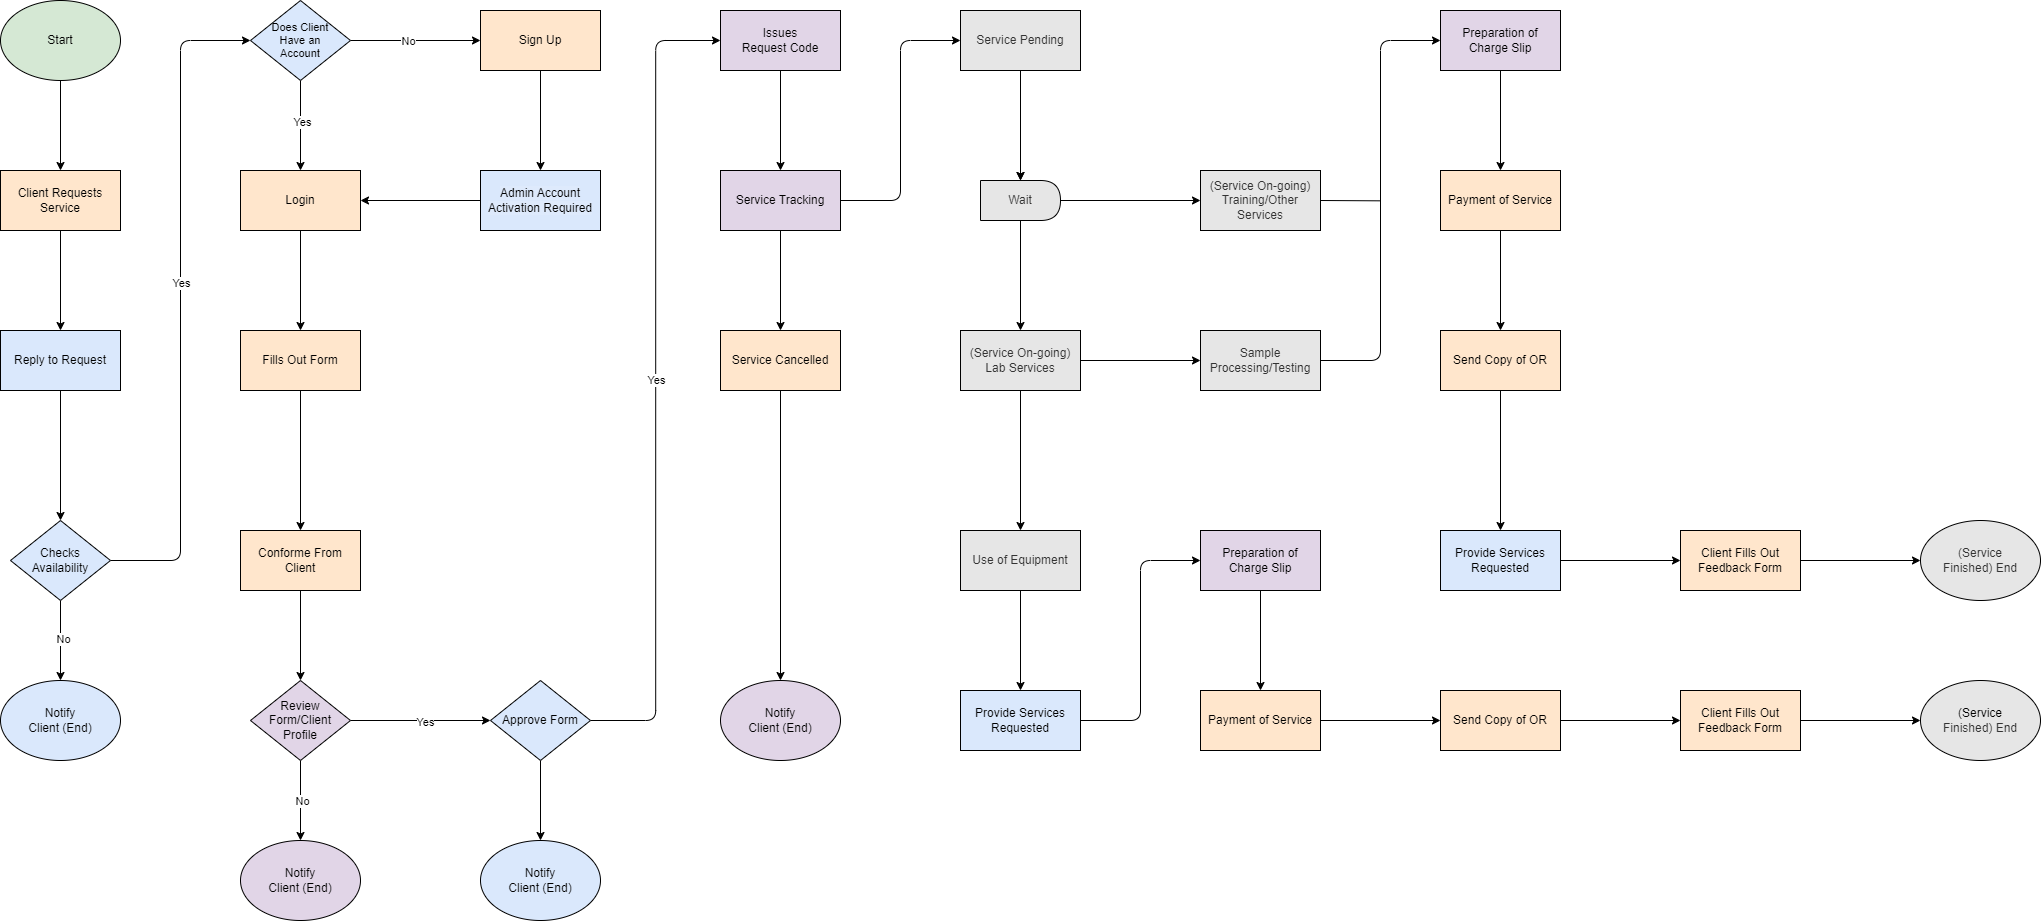
\includegraphics[width=1\textwidth]{process_flow_diagram.png}
	\caption{Process Flow Diagram}
	\label{fig:process_flow}
\end{figure}

\subsection{Context Model}

\figref{fig:context_model} illustrates the interactions between the system and both internal and external entities. It shows how the system communicates with different stakeholders, including client, staff, director, and university researcher. The model also outlines how information flows from entities to the system and vice versa, showing how it works and its role within the institution.

\textbf{Clients} will primarily interact with the system to make service inquiries or submit requests related to the services offered by the UPV RRC. They might also provide feedback or report issues based on their interactions with the system or their overall experience on transacting with the UPV RRC.

For the \textbf{University Researchers}, they can use the system to oversee any laboratory-related requests, such as assessing, approving and terminating requests. Additionally, they can also use the system to release the results of the service rendered, if the client wishes to have it in softcopy. 

Similarly, \textbf{TECD Staff} can use the system to oversee, equipment or facility rental related requests. This also includes assessing, approving, and terminating request. 

For the \textbf{Admin Staff}, the system will provide oversight on the ongoing transactions. Admin staff ensure that users from various roles perform their duties effectively by managing accounts, permissions, and system-wide configurations. Like the university researchers and TECD staff, they also have access on the service-related requests and have an ability to assess, approve, and terminate transactions or requests.

\newpage

\begin{figure}[h]
	\centering 
	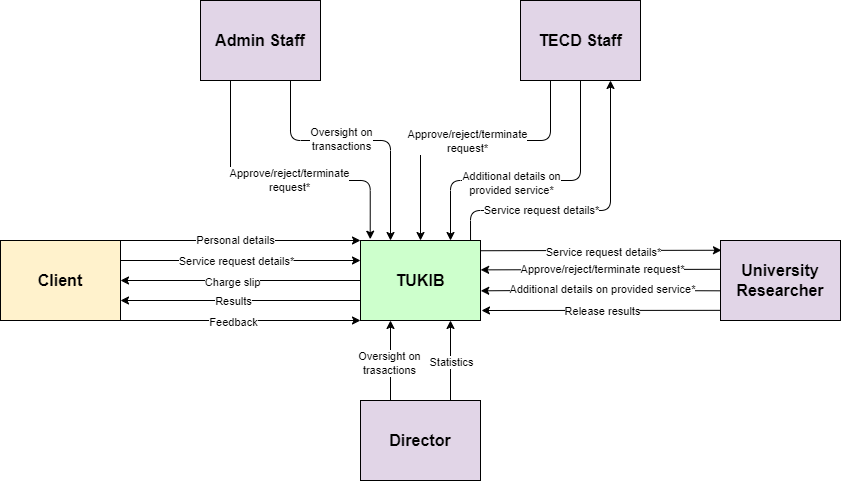
\includegraphics[width=1\textwidth]{context_model.png}
	\caption{Context Model}
	\caption*{\textit{Note:} Some data flow names (e.g., \texttt{Service request details}) appear more than once to represent shared interactions across multiple entities. An asterisk (*) indicates a repeated data flow for visual clarity.}
	\label{fig:context_model}
\end{figure}

\subsection{Use Case Diagram}

Figures \ref{fig:use_case_client}, \ref{fig:use_case_admin}, \ref{fig:use_case_director}, and \ref{fig:use_case_staff} present the use case diagrams of the system, which visually represent the key interactions between different types of users and the system in the service management cycle of the UPV RRC. The diagrams highlight the various roles and their associated tasks in managing service requests.

\newpage

\begin{figure}[h]
	\centering
	\begin{minipage}{0.30\textwidth}
		\centering
		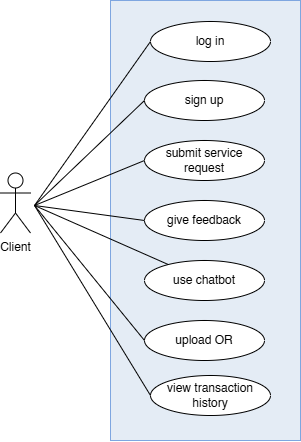
\includegraphics[width=\textwidth]{use_case_client.jpg}
		\caption{Use Case Diagram (Client interface)}
		\label{fig:use_case_client}
	\end{minipage}%
	\hfill
	\begin{minipage}{0.32\textwidth}
		\centering
		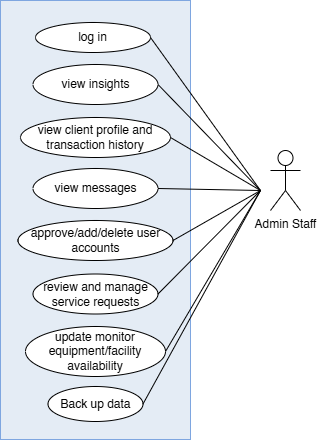
\includegraphics[width=\textwidth]{use_case_admin.jpg}
		\caption{Use Case Diagram (Admin interface)}
		\label{fig:use_case_admin}
	\end{minipage}
	
	\vspace{0.5cm} % Add some vertical space between the rows
	
	\begin{minipage}{0.30\textwidth}
		\centering
		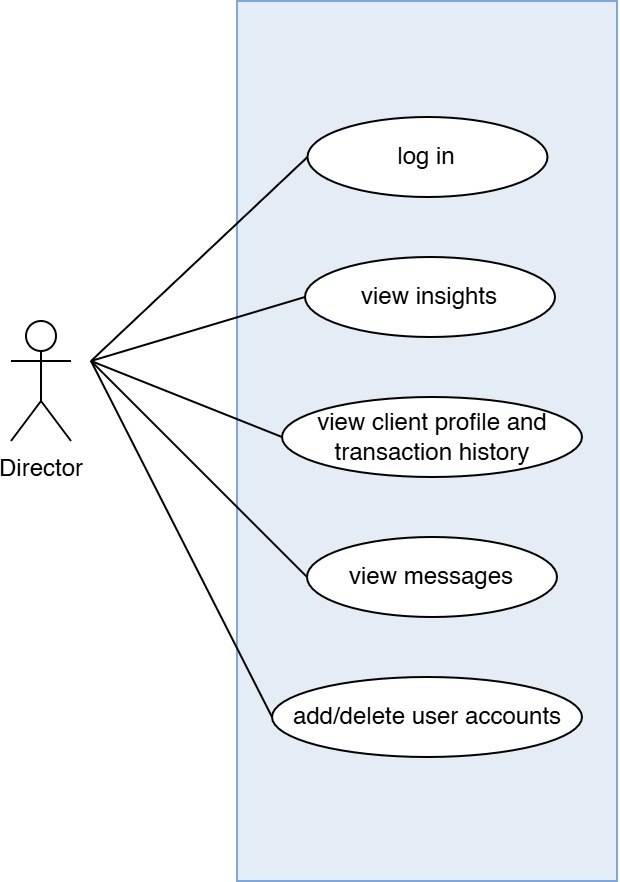
\includegraphics[width=\textwidth]{use_case_director.jpg}
		\caption{Use Case Diagram (Director interface)}
		\label{fig:use_case_director}
	\end{minipage}%
	\hfill
	\begin{minipage}{0.30\textwidth}
		\centering
		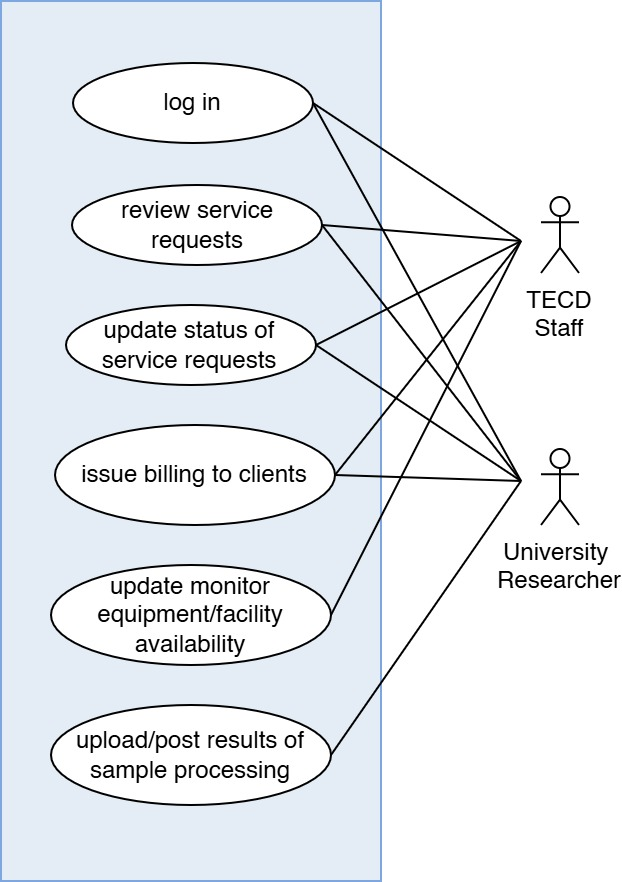
\includegraphics[width=\textwidth]{use_case_staff.jpg}
		\caption{Use Case Diagram (TECD and UR interface)}
		\label{fig:use_case_staff}
	\end{minipage}
\end{figure}

\newpage

\subsection{Database Diagram}

The database design for TUKIB revolves around tracking and managing various service-related data through several interrelated entities to ensure efficient storage and retrieval. As shown in \figref{fig:database}, the system consists of multiple interconnected tables that support core functionalities of laboratory operations, service requests, and user management.

The \textbf{usersTable} stores essential information about system users, including names, contact details, roles, and associated laboratories, as referenced from the \textbf{laboratories} table. This linkage enables the system to group users by their laboratory affiliations.

When a user initiates a service, a corresponding entry is created in the \textbf{serviceRequestTable}, which records the requester, service type (e.g., equipment rental, facility rental, sample processing, or training), status, and associated documentation such as receipts or results. Each request may be approved or rejected by another user, establishing a self-referential relationship within the same table.

To support different request types, there are specialized tables: the \textbf{equipmentRentalRequests}, \textbf{facilityRentalRequests}, \textbf{sampleProcessingRequests}, and \textbf{trainingRequests}. Each of these tables references the \textbf{serviceRequestTable} and captures detailed, request-specific data such as equipment settings, facility schedules, sample details, or training requirements.

Resource data is maintained separately. The \textbf{equipmentsTable} stores equipment metadata including model, quantity, and laboratory assignment, while the \textbf{facilitiesTable} contains information about available facilities, capacity, and resources. 

The \textbf{calendar} table manages the scheduling aspect of the system, enabling time-based coordination for events and date restrictions. It supports both general and specific calendars dedicated for scheduling of each facilities, laboratories, and equipment.

User authentication and security are handled through the \textbf{user\_tokens} table, which manages token-based login sessions and expiration tracking.

Additionally, the schema includes unconnected tables by design. The \textbf{messagesTable} stores public inquiries sent via the system's contact form, allowing non-registered visitors to send messages. Since it is intentionally decoupled from the user system, it does not reference the \textbf{usersTable}. Similarly, the \textbf{feedback\_table} is designed for anonymous client input and does not store identifiable user data. This supports unbiased service evaluation while protecting user privacy.

Overall, the schema promotes modularity and data integrity with clear separations between request types, resource tracking, and additional functions such as messaging and feedback.

\newpage

\begin{figure}[h]
	\centering 
	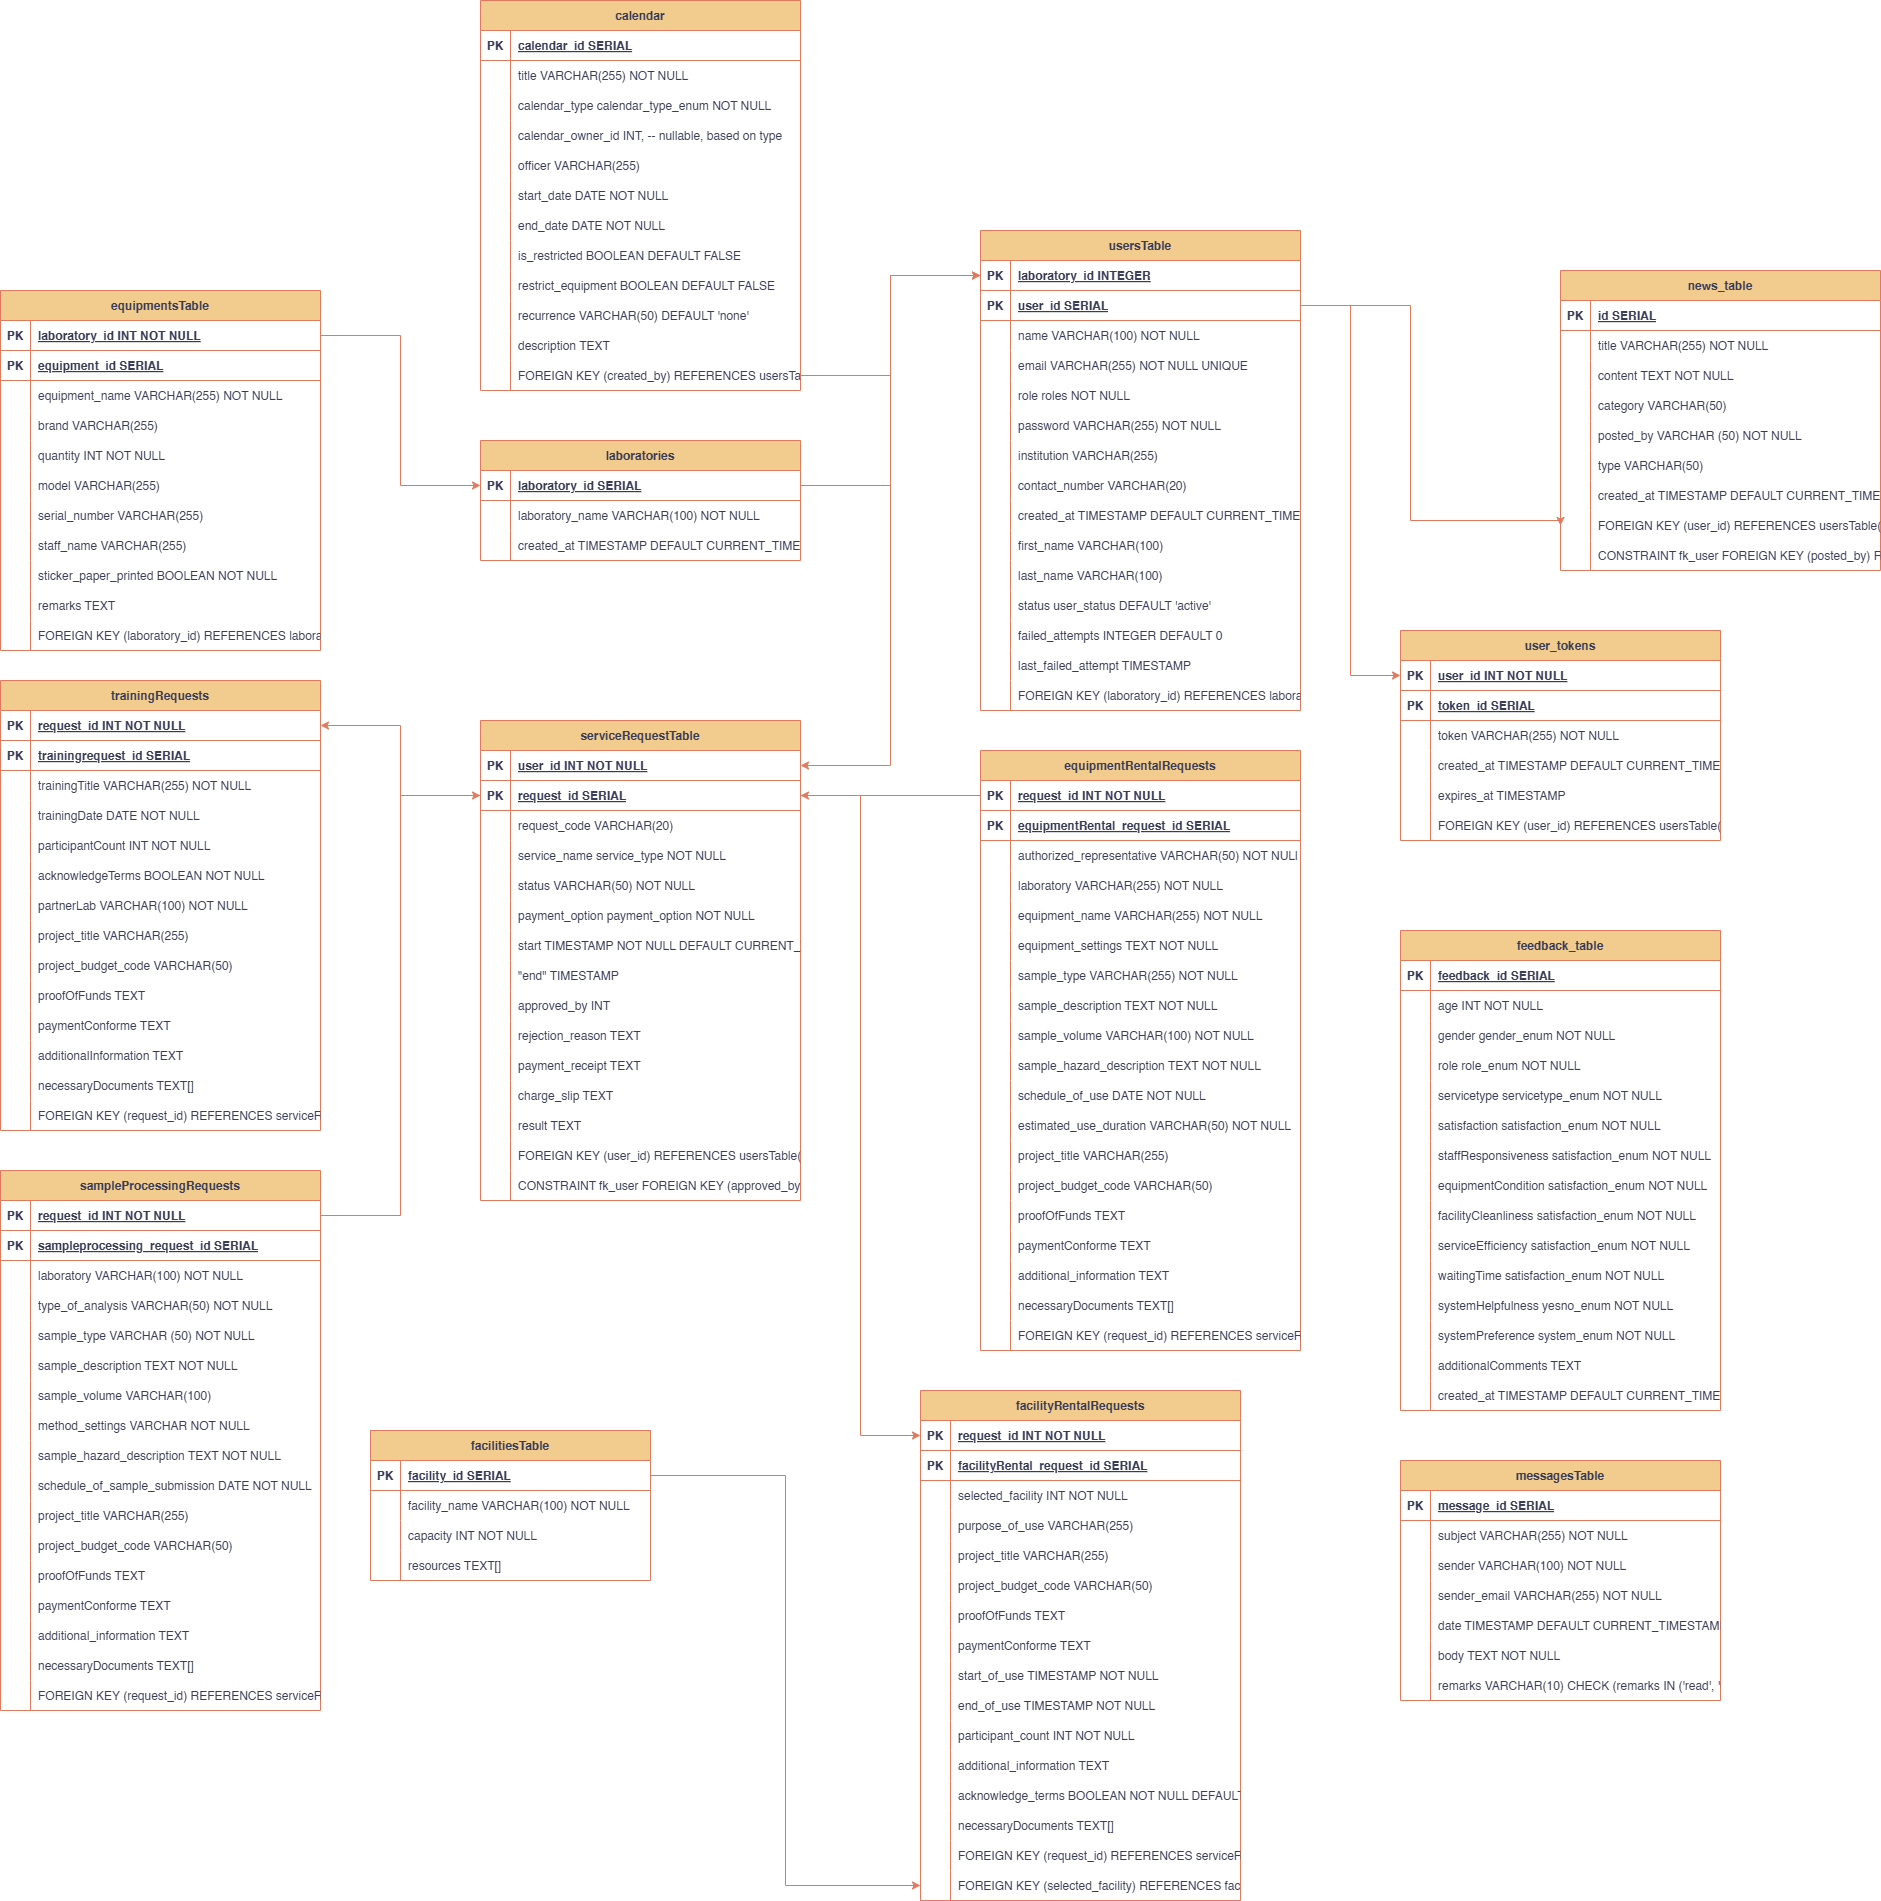
\includegraphics[width=1\textwidth]{database2.png}
	\caption{Database Design Diagram}
	\label{fig:database}
\end{figure}

\section{Chatbot architecture}

This section outline the architecture of the Rasa framework, as well as, the necessary information on how the chatbot is developed.

\subsection{Rasa Chatbot Architecture}

The chatbot for the system was created using the Rasa framework. Rasa is an open source conversational AI framework that allows developers to build, deploy, and improve AI-powered chatbots and virtual assistants. \figref{fig:rasa_architecture} shows the details about the architecture of Rasa chatbot design. Specifically, this study utilized the Open Source framework of Rasa.

There are two main components in Rasa Open Source architecture namely: Rasa NLU and Rasa Dialogue Policies. The Rasa NLU, shown as NLU pipeline in the figure, is like the primary senses of the chatbot which receive the input from the users. It identifies, classifies, and extracts the intents and entities from the given input. It is also responsible for choosing and retrieving the appropriate response to the user. 

The dialogue management also called the Rasa Core, shown as Dialogue Policies in the figure, decides the next action in a conversation based on the context of the conversation. Rasa SDK is an action server which is responsible for running custom actions. The Tracker store is where the conversations are stored. The chatbot saves the context which helps give personalized interactions with the user as it learns over time. Rasa also uses a ticket lock mechanism to ensure that incoming messages for a given conversation ID are processed in the right order, and locks conversations while messages are actively processed. This allows for multiple Rasa servers to be run in parallel. File system consists of Models and Training data needed for the functionality of the chatbot.

\newpage

\begin{figure}[h]
	\centering 
	\includegraphics[width=1\textwidth]{RASA_architecture.png}
	\caption{Rasa Open Source Chatbot Architecture}
	photo from https://rasa.com/docs/rasa/arch-overview/
	\label{fig:rasa_architecture}
\end{figure}

\subsection {Conversation Processing}

Rasa mainly includes three stages in its conversation processing. They are:

\begin{itemize}
	\item \textbf{NLP pipeline (Natural Language Processing)}
	
	The input or message is given by the user in this stage. The chatbot mainly tries to understand the context of the user’s message and meaningful information is extracted. This stage involves tokenization, intent and entity recognition, and featurization. The extracted information is then mapped or matched with the training data.
	
	\item \textbf{Dialogue management (Response selection stage)}
	
	Once the input is processed by the NLP pipeline, it proceeds to the dialogue management stage. This stage involves decision-making about how the bot should respond based on the user’s given input and the context of the conversation. 
	
	\item \textbf{Response Generation / Output}
	
	Once the appropriate response or action has been determined, the final stage is to generate the bot’s response to the user.  There are two main approaches for generating these responses. First is the template-based responses which are the pre-defined response templates based on the extracted intent and entities from the user’s message. These responses are static and are typically used for simple and predictable replies. Another is the custom action. This is for complex responses, such as calling an API or performing specific logic. For example, the chatbot will call from the backend to fetch service details or event schedules, and then dynamically generate a response based on the result.
	
\end{itemize}

\subsection{Model Training}

For this study, the training data used was in the form of conversations between the RRC staff and clients. The data collection was done with the help of RRC staff to ensure its accuracy and validity. The gathered data was used to train Rasa’s NLU model, allowing it to recognize user intents and extract relevant information accurately. As per Rasa’s capability, continuous use of the chatbot further trains the model, allowing it to learn from interactions and improve its understanding over time. This ongoing training process will enhance the chatbot’s performance, ensuring it becomes more adept at addressing user needs and providing relevant and more accurate responses as it accumulates more data from real-world users.

\subsection {Limitations of Rasa}

Rasa is a powerful open-source framework for building conversational AI applications, but like any other technology implemented, it also has its limitations. The first is that Rasa has a higher learning curve. To be able to use Rasa, developers must know Python, machine learning concepts, and experience in natural language processing. Without these Rasa wont be set up and utilized effectively. 

Another is how Rasa is highly dependent on training data. In another view, this may help the developers customize the responses and conversations to their specific needs. However, when training is poorly done and insufficient data is given, this results in low chatbot accuracy. This backfires and counters the purpose of chatbots in providing accurate assistance. Hence, extensive training data to account for various scenarios and user inputs is needed for proper context modeling.

\section{Chatbot Design and Development}
This section presents the design of the chatbot component for the TUKIB system. It details the structure, conversational flow, and the integration of natural language processing elements used to support user interactions and service inquiries.

\subsection{Entities and Intents}

From the data gathering phase, the developers were able to identify common user queries and specific service requirements needed for the development of the chatbot. The collected data was used to construct the intents and entities which are essential for the chatbot’s functionality. 

Intents represent the goal the users want to achieve when interacting with the chatbot (e.g., ``start consultation,” ``ask about lab rental procedures,” ``inquire about service status”). The intents are divided into greeting, general, service requests, frequently asked questions, feedback, and end or closing message. On the other hand, entities are specific pieces of information that the chatbot needs to get from the user in order to fulfill a task. For example, the chatbot needs to know the name of the equipment and desired time for renting in order to indicate the equipment's availability. 

\subsection{Conversation Flow}

\figref{fig:chatbot_flow} illustrates the conversation flow for TUKIB's chatbot, named LIRA— short for Learning, Innovation, and Research Assistant. LIRA will be accessible throughout the entire website, ensuring that all users, whether logged in or not, can obtain support whenever needed. Users can initiate a chat with LIRA via a persistent button that remains visible across the site or by selecting the dedicated “New Service Request” button found on the user dashboard.

\newpage

\begin{figure}[h]
	\centering 
	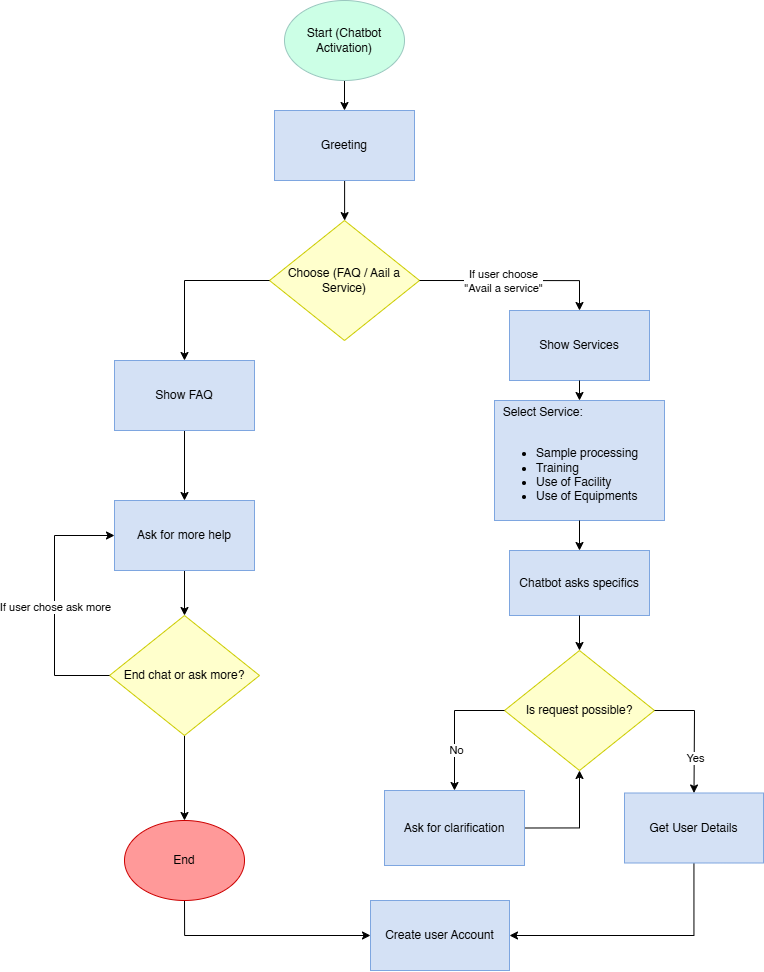
\includegraphics[width=0.70\textwidth]{chatbot_flow.png}
	\caption{LIRA Conversation Flow}
	\label{fig:chatbot_flow}
\end{figure}

The structure of the chatbot is centered around a conversational flow that guides users through various tasks, from inquiries to service request consultations. The chatbot’s design consists of the following core components:

\begin{itemize}
	\item \textbf{Welcome Greeting}
	
	Present a welcome message where the chatbot greets users with a friendly introduction and offers assistance, presenting options such as ``Service Inquiry'' and “Frequently Asked Questions/FAQs.” 
	
	\item \textbf{Flow for Service Inquiry}
	
	If the user chooses the option “Service Inquiry,” the chatbot will ask a follow-up question to identify which service the user wishes to inquire about. Sample service choices include sample processing,  lab equipment rental, etc. Then, the chatbot uses the user's answer details to present accurate information about each service.
	
	\item \textbf{Flow for Consultation}
	
	The flow for consultation is designed to facilitate user inquiries about the services they wish to avail. As the primary purpose of the chatbot, this interaction allows users to ask questions about the services offered by RRC. When a user expresses interest, the chatbot engages by asking for specific details related to their request. For instance, if a user inquires about sample processing (e.g., the type of sample and processing methods needed), the chatbot will guide them through the details. This interactive process ensures that users receive tailored information while the chatbot gathers necessary details to asses service feasibility.
	
	\item \textbf{Flow for General Questions / FAQ}
	
	The chatbot should be able to answer and handle frequently asked questions by clients. These would include questions about general services, rental pricing methods, facility rental processes, etc.
	
	\item \textbf{Error Handling}
	
	Chatbot failures will lead to conversational dead ends if not dealt with properly. Thus, negating the main purpose of chatbot in this system which is to provide efficient customer service. To address this, the chatbot will have a fallback mechanism whenever an input from user was unexpected or a system error occurs. For example, if the chatbot cannot understand the user input, there will be rules on how the chatbot would handle this situation. Sample fallback methods would be redirecting the conversation to a live agent. Another option would be presenting friendly-toned error messages to the users, letting them know that the chatbot is having trouble understanding their input.
	
	Sample error messages include “Sorry, I didn't catch that. Could you rephrase your question?” or “I'm sorry, I have a hard time understanding. Could you please rephrase your query?” and “I'm sorry, but what you're asking is not clear to me. Could you paraphrase it?”
	
\end{itemize}

\section{Storage and Database Architecture}

TUKIB utilizes PostgreSQL as its database management system and implements table partitioning to efficiently manage data and improve system performance. Instead of using separate databases for active and archived data, partitioning divides large tables based on a date range, such as service request dates, allowing recent records to be accessed quickly while older records are stored in separate partitions.

This approach enables the system to maintain fast and responsive queries on current data while still preserving access to historical information without the overhead of managing multiple databases. Records older than one year are automatically moved to archived partitions through scheduled maintenance tasks, reducing the load on active partitions and ensuring continued system efficiency.

Additionally, regular automated backups are scheduled using PostgreSQL’s built-in backup tools to secure both active and archived partitions. These backups ensure data durability and support quick recovery in case of system failures, minimizing potential disruptions to RRC’s service delivery.

\section{Development Tools}

\subsection{Hardware}

The hardware requirements for the development of the system include a computer or laptop with the following specifications:

\begin{itemize}
	\item Processor: Intel Core i5, its equivalent on other brands or higher
	\item RAM: 6GB or higher
	\item Storage: 200GB SSD or more for faster data access and retrieval
	Operating System: Windows 10 or higher, macOS, or Linux
\end{itemize}

These specifications are necessary to ensure smooth development and testing of the system, especially when handling large datasets and concurrent processes.

\subsection{Software}

TUKIB will be developed using a range of modern software tools tailored to meet the specific needs of the research center’s workflow automation and data management processes.

\begin{itemize}
	\item \textbf{HTML5, CSS, Bootstrap, and ReactJS}
	
	These technologies were used for front-end development of the system. HTML5 structured the webpages, CSS was responsible for the visual styling, Booststrap for UI $ $flexibility, and ReactJS enabled dynamic and interactive user interfaces.
	
	\item \textbf{PostgreSQL}
	
	For backend development, PostgreSQL was used as the database management system, offering robust data storage, querying, and management capabilities.
	
	\item \textbf{Rasa Framework}
	
	Rasa used for the chatbot development. It allowed the creation of a conversational AI system which handled the service requests, queries, and management capabilities of the system.
	
	\item \textbf{Figma}
	
	Figma wwas utilized for designing the UI/UX of the system. Figma allowes design collaboration, which enabled the team to create the system prototype, wireframe, and mock-up interfaces before implementation, ensuring a user-friendly experience for both clients and researchers.
	
	\item \textbf{VS Code}
	
	Visual Studio Code (VS Code) was the primary code editor that was used to develop the system. Its features, such as syntax highlighting, extensions, integrated Git, and debugging tools, made it the most suitable environment for writing and testing front-end and back-end code.
	
	\item \textbf{Github}
	
	GitHub was used to facilitate for version control and collaboration thoughout the development of the system. The project code was stored in repositories, allowing the team to manage changes, track progress, and collaborate effectively. It also served as a backup and source for future development or modification.
	
\end{itemize}
